
% Proposta TCC1 - Professora Ana Cristina B. Kochem Vendramin (cristina@dainf.ct.utfpr.edu.br, criskochem@utfpr.edu.br)

\documentclass{normas-utf-tex_07_2012} %Estilo de Formato criado pelo Prof. Hugo Vieira Neto (hvieir@utfpr.edu.br)
%Se você ainda não conhece o latex, comece olhando o site do Prof. Hugo --> http://pessoal.utfpr.edu.br/hvieir/orient/

%\documentclass[twoside,openright]{normas-utf-tex} %openright = o capitulo comeca sempre em paginas impares

%\usepackage[alf,abnt-emphasize=bf,bibjustif,recuo=0cm, abnt-etal-cite=2, abnt-etal-list=99]{abntcite} %configuracao das referencias bibliograficas.
\usepackage[alf]{abntex2cite}	% Citações padrão ABNT
\usepackage[brazil]{babel} % pacote portugues brasileiro
\usepackage[utf8]{inputenc} % pacote para acentuacao direta
\usepackage{amsmath,amsfonts,amssymb} % pacote matematico
\usepackage[pdftex]{graphicx} % pacote grafico
\usepackage{times} % fonte times
\usepackage{a4wide}
\usepackage[a4paper]{geometry} %define papel a4...
\geometry{left=3cm,right=2cm,top=3cm,bottom=2cm} % ...e suas margens
\usepackage{tabularx,multirow,longtable} %pacotes para mesclar linhas/colunas; tabelas grandes
\usepackage{fancyhdr} % altera cabeçalhos
\usepackage[T1]{fontenc} % acentuação direto no texto
\usepackage{ae} % “Almost European”: aumenta a qualidade do pdf final
\usepackage{rotating} % faz rotações de tabelas e figuras
\usepackage{indentfirst} % tabula a primeira linha do parágrafo
\usepackage[hang,small,bf]{caption} % legendas; nome "tabela" ou "figura" em negrito
\usepackage{caption3}
\usepackage{setspace} % ajuste do espaço entre-linhas
%\usepackage{algorithm}
\usepackage{subfig}
\usepackage{float} % posicionamento das figuras
\usepackage{subfloat}
%\usepackage{arydshln}
%\usepackage[backend=biber]{biblatex}
\makeatletter
%\renewcommand{\ALG@name}{Algoritmo}
%\usepackage{algorithmic}

%para a hifenacao funcionar é necessario fazer a seguinte modificacao
%Clique em Iniciar -> Programas -> MikTeX -> MiKTeX options Vá em Languages e marque a caixa português.

%hifenacoes customizadas
\hyphenation{mo-de-lar re-no-vá-veis re-pre-sen-tar re-pre-sen-ta-ção la-te-rais res-pec-ti-vos re-a-ção re-a-li-zan-do o-pe-ra-ções cons-tan-te di-fe-ren-tes tem-pe-ra-tu-ra ex-tre-mi-da-de ter-mo-di-nâ-mi-ca trans-es-te-ri-fi-ca-ção In-ter-net}

%%%% Comandos introduzidos para controlar as alteracoes no fonte%%%%%%%%%%%%%%%%%
% assigning colors to comments of each author
\usepackage{color}
\newcommand{\cris}[1]{\textcolor{blue}{#1}} %texto final
\newcommand{\crisC}[1]{[\textcolor{blue}{#1}]} % comentário entre colchetes
\newcommand{\ane}[1]{\textcolor{red}{#1}} %texto final
\newcommand{\aneC}[1]{[\textcolor{red}{#1}]} % comentário entre colchetes
%%%%%%%%%%%%%%%%%%%%%%%%%%%%%%%%%%%%%%%%%%%%%%%%%%%%%%%%%%%%%%%%%%%%%%%%%%%%%%%%%%%%%%

% ---------- Preambulo ----------
\instituicao{Universidade Tecnológica Federal do Paraná} % nome da instituicao
\programa{Departamento Acadêmico de Informática} % nome do programa ou departamento
\area{Curso de Engenharia de Computação} % área ou curso

\documento{Trabalho de Conclusão de Curso} % [Trabalho de Conclus\~ao de Curso] ou [Disserta\c{c}\~ao] ou [Tese]
\nivel{Graduação} % [Gradua\c{c}\~ao], [Especializa\c{c}\~ao], [Mestrado] ou [Doutorado]
\titulacao{Engenheiro} % [Engenheiro], [Tecn\'ologo], [Bacharel], [Mestre] ou [Doutor]

\titulo{\MakeUppercase{Utilização de aplicativo móvel e \textit{crowdsourcing} para rastreio de ônibus}} % titulo do trabalho em portugues
\title{\MakeUppercase{}} % titulo do trabalho em ingles

\autor{Gionatta Marcon Mocellin} % autor do trabalho
\autordois{Giusepe Pietro Niquele}
\cita{MOCELLIN, Gionatta Marcon. NIQUELE, Giusepe Pietro} % sobrenome (maiusculas), nome do autor do trabalho

\palavraschave{Incluir as palavras-chave em português} %substituir pelas palavras-chave relacionadas ao seu tema de pesquisa
\keywords{Incluir as palavras-chave em inglês} % incluir palavras-chave em inglês

\comentario{Proposta de \UTFPRdocumentodata\ de Engenharia de Computação apresentado ao \UTFPRprogramadata\ da \ABNTinstituicaodata\ como requisito parcial para obtenção do título de ``\UTFPRtitulacaodata\ em Computação''.} %\\ \'Area de Concentra\c{c}\~ao: \UTFPRareadata.}

\orientador[Orientadora:]{Prof$^a$. Dr$^a$. Ana Cristina Kochem Vendramin} % <- no caso de orientadora, usar esta sintaxe
\coorientador[Co-orientadora:]{\hspace*{3mm}Prof$^a$. Dr$^a$. Anelise Munaretto \newline \hspace*{3mm}Fonseca} % <- no caso de co-orientadora, usar esta sintaxe


\local{Curitiba} % cidade
\data{2014} % ano
\setcounter{tocdepth}{4} % para numeração das seções
\setcounter{secnumdepth}{4}

\numberwithin{equation}{chapter} %
%\numberwithin{table}{chapter} %
%\numberwithin{figure}{chapter} %

\makeatletter  %% this is crucial
 \renewcommand\subsubsection{\@startsection{subsubsection}{3}{\z@}%
                        {-2\p@ \@plus -0.5\p@ \@minus -0.5\p@}%
                        %{8\p@ \@plus 4\p@ \@minus 4\p@}%     <-- this is copied from the subsection command
                        {2\p@ \@plus 1\p@ \@minus 1\p@}%     <-- this is copied from the subsection command
                        {\normalfont\normalsize\bfseries\boldmath
                         \rightskip=\z@ \@plus 8em
 \pretolerance=10000 }}
\makeatother   %% this is crucial

%---------- Inicio do Documento ----------
\begin{document}

\capa % geracao automatica da capa

\folhaderosto % geracao automatica da folha de rosto

% dedicatória (opcional)
%\begin{dedicatoria}
% Texto da dedicat\'oria.
%\end{dedicatoria}

% agradecimentos (opcional)
%\begin{agradecimentos}
% Texto dos agradecimentos.
%\end{agradecimentos}

% epigrafe (opcional)
%\begin{epigrafe}
%\end{epigrafe}

%resumo
%\begin{resumo}

%Incluir o resumo aqui

%\end{resumo}

%abstract
%\begin{abstract}

%Include the abstract here

%\end{abstract}

% listas que recomenda-se a partir de 5 elementos
%\listadefiguras % geracao automatica da lista de figuras

%\listadetabelas % geracao automatica da lista de tabelas

\listadesiglas % geracao automatica da lista de siglas
%Constituída de uma relação alfabética das abreviaturas e siglas utilizadas no texto, seguido das palavras ou expressões correspondentes grafadas por extenso. Utilizada apenas se houver siglas.

%\listadesimbolos % geracao automatica da lista de simbolos
%Elaborado de acordo com a ordem apresentada no texto, seguido do significado correspondente. Utilizada apenas se houver símbolos.

% sumario
\sumario % geracao automatica do sumario

%---------- Inicio do Texto ----------

\setcounter{page}{3} % *** Necessário arrumar manualmente antes de imprimir

% O label serve para referenciar o capítulo quando necessário
\chapter{Introdução}\label{cap:introducao}

O conceito de \textit{Smart Cities} (Cidades Inteligentes, em tradução livre) é um sustentáculo elementar para o desenvolvimento urbano sustentável. De certa forma, ele poderia contribuir na solução de diversos problemas críticos, originados a partir da urbanização de grandes cidades como congestionamentos, poluição do meio ambiente, e os limites dos recursos naturais. \cite{pan2013}.
 
Um outro aspecto do conceito de cidades inteligentes a ser considerado, é a importância crescente das tecnologias digitais para um futuro sustentável. Assim sendo, destaca-se seis principais áreas, nas quais essas inovações digitais tem a competência para fazer a diferença: vida inteligente, governança inteligente, economia inteligente, ambiente inteligente, pessoas inteligentes e mobilidade inteligente \cite{schuurman}.
 
Com o uso da tecnologia da informação e comunicação (do inglês {\sigla{ICT}{\emph{Information and Communication Technology}}, \emph{Information and Communication Technology},}) a  análise e mineração de dados de sensoriamento grande cidades é um passo importante para considerá-las uma cidade inteligente. Por exemplo, informações sobre a mobilidade dos veículos e pessoas tornaram-se temas em voga nos últimos tempos  devido à prevalência do \sigla{GPS}{\emph{Global Positioning System}} (\emph{Global Positioning System}) e outras tecnologias de localização. Esse conhecimento sobre a cidade e seus habitantes poderá trazer benefícios nas áreas de transporte, planejamento urbano, saúde pública, segurança pública e comércio \cite{pan2013}.
 
Embora as ações de sensoriamento e mineração dos dados seja de imprescindível importância, algo deve ser feito para transformar esses dados em informações. Nesse sentido, uma abordagem interessante para a resolução desta questão consiste no conceito de \textit{crowdsourcing} \cite{schuurman}.

\citeonline{Howe2006} caracteriza \textit{crowdsourcing} como o fenômeno no qual várias pessoas comuns dedicam seu tempo livre na busca de soluções para um problema de interesse coletivo. Isto posto, a massificação dos chamados \textit{smartphones} e o advento de redes móveis e sem fio tais como o 3G e o WiFi e recentemente, o 4G, permitem que pessoas fiquem conectadas a maior parte do tempo, em qualquer lugar. Dentre os inúmeros benefícios que os \textit{smartphones} fornecem, a possibilidade de troca de informações entre usuários é uma delas, bem como a aplicação do conceito de \textit{crowdsourcing}.

Considera-se o seguinte cenário: uma pessoa que acabou de chegar em um ponto de ônibus, deseja saber onde o mesmo se encontra. Questões como ``será que o ônibus está chegando?'', ``será que vai demorar?'' ou ``será que o ônibus estragou?'' são bastante comuns. Mas como descobrir suas respostas? Infelizmente, não é possível respondê-las apenas com a tabela de horários de chegada dos ônibus, disponível nos terminais e no \textit{site} da \sigla{URBS}{Companhia de Urbanização e Saneamento de Curitiba} (Companhia de Urbanização e Saneamento de Curitiba).

Nesse sentido, é proposto nesse documento uma solução possível para esse quesito. A ideia básica é a construção de um aplicativo que alie conceitos, tanto de \textit{Smart Cities} quanto de \textit{crowdsourcing}, no qual informações em tempo real sobre o transporte coletivo, especificamente no que compete o estado atual de uma linha de ônibus, sejam disponibilizadas aos usuários.

%breve estado da arte

Alguns aplicativos para dispositivos móveis foram desenvolvidos com o objetivo de prover, ao usuário, informações referentes ao transporte público. Um dos aplicativos mais recentes é o chamado ``Busão Curitibano'', lançado em 2013\footnote{Para mais informações sobre o aplicativo, consultar notícia da Gazeta do Povo, disponível em:  http://www.gazetadopovo.com.br/vidaecidadania/conteudo.phtml?id=1377575}. Os desenvolvedores -- e também os usuários do aplicativo -- encontraram algumas resistências por parte da URBS, pois o aplicativo usava a base de dados do transporte coletivo. Devido aos inúmeros acessos, acabava derrubando o servidor da URBS e tornando o serviço de acompanhamento de ônibus indisponível.

Outro aplicativo semelhante foi desenvolvido por \citeonline{sujatha}. Os autores propuseram um sistema chamado \sigla{MBTS}{Mobile Bus Tracking System} (\emph{Mobile Bus Tracking System}) que ajuda qualquer pessoa a obter informações de um determinado ônibus sem fazer ligações ou perturbar passageiros com mensagens \sigla{SMS}{\emph{Short Message Service}} (\emph{Short Message Service}). %O sistema funciona com, basicamente, três atores: os passageiros, os “coordenadores” do ônibus e as pessoas que estão aguardando em um ponto. Todos os atores necessitam de um \textit{smartphone} com sistema operacional Android conectado à Internet. Continuamente, os passageiros e os ``coordenadores'' alimentam um banco de dados com informações sobre o ônibus, tais como as coordenadas do veículo, as quais estarão disponíveis para as pessoas que estão aguardando pelo ônibus.
Um banco de dados é utilizado para armazenar informações sobre os ônibus (por exemplo, as coordenadas do veículo), as quais estarão disponíveis para acesso através de um aplicativo Android..

\section{Justificativa}

A utilização de uma arquitetura centralizada, estilo cliente--servidor é um ponto comum nos dois trabalhos relacionados. Em ambos, nota-se que a arquitetura encontra-se em uma relação n:1, ou seja, vários clientes para um único servidor. Alguns dos problemas que podem surgir nesse tipo de arquitetura é que o servidor pode ficar sobrecarregado e eventualmente ficar indisponível devido ao grande número de usuários utilizando o serviço, como foi o caso do ``Busão Curitibano''. Além disso, nesse caso, o servidor utilizado não é de propriedade dos desenvolvedores, mas sim da Urbs. Caso a companhia deseje interromper o serviço de fornecimento de dados, o ``Busão Curitibano'' perde sua utilidade. Isso não constitui um problema para o MBTS, pois o mesmo concentra as informações em um servidor próprio, mantido pelos próprios desenvolvedores.

Sendo assim, a principal motivação para o desenvolvimento deste projeto é implementar um aplicativo de acompanhamento de ônibus para dispositivos móveis -- \textit{smartphones} -- que utilize uma rede descentralizada. Nela, os próprios usuários são os nós, que compartilharão informações entre si. Para tal, utilizar como referência o aplicativo móvel ``Waze''\footnote{Uma análise do aplicativo pode ser encontrada em http://www.techtudo.com.br/tudo-sobre/waze.html}, que implementa uma espécie de comunidade para mapeamento do trânsito em tempo real. Através do ``Waze'', cerca de 40 milhões de usuários compartilham informações, no mundo todo \cite{techtudoWaze}.

Além disso, usufruir do recurso de GPS, já utilizado nos ônibus de Curitiba, para fornecer aos usuários a posição dos veículos.

\section{Objetivo geral}

Desenvolver um aplicativo para \textit{smartphones} que rodam sobre o sistema operacional Android, para acompanhamento de ônibus em Curitiba, unindo idéias de aplicativos já existentes como o ``Waze'' e o ``Busão Curitibano'', e o conceito de \emph{crowdsourcing}.

\section{Objetivos específicos}

\begin{itemize}
\item Desenvolver um aplicativo, para \textit{smartphones}, para acompanhamento de ônibus da rede de transporte de Curitiba;
\item Estudar e implementar no aplicativo o conceito de \textit{crowdsourcing}, para permitir que usuários colaborem entre si com informações pertinentes, através de \textit{feedbacks} pré-definidos no aplicativo;
\item Desenvolver o aplicativo para que o mesmo seja executado sobre uma plataforma que não exija custos de desenvolvimento;
\item Implementar uma arquitetura de rede descentralizada, a fim de evitar problemas como sobrecarga de servidor.
\end{itemize}

\section{Estrutura e organização}

O presente documento encontra-se organizado da seguinte forma. O capítulo 1 apresenta a introdução, com a formulação do problema, justificativa do projeto, objetivo geral e específicos do mesmo. O capítulo 2 apresenta o levantamento bibliográfico, importante para fundamentar o projeto e fornecer um embasamento. A metodologia, que descreve as etapas de desenvolvimento pelas quais o projeto percorrerá, é apresentada no capítulo 3. Os recursos para desenvolvimento do projeto e a viabilidade do mesmo, são apresentados nos capítulos 4 e 5, respectivamente. Por fim, conclusões pertinentes ao desenvolvimento do projeto, tais como dificuldades esperadas e horizontes de projeto, são apresentados no capítulo 6.

\chapter{Levantamento Bibliográfico}\label{cap:levbibliog}

Este capítulo apresenta uma breve introdução à \textit{Smart Cities}, \textit{Crowdsourcing}, contexto atual do desenvolvimento de programação voltada a aplicativos de transporte público e demais tópicos relativos ao desenvolvimento do trabalho.

\section{\textit{Smart Cities}}

O conceito de Cidades Inteligentes e o respectivo aumento no seu uso, pode ser reconhecido como o resultado do alto crescimento das tecnologias digitais na intenção de garantir um futuro sustentável. Embora o conceito seja empregado normalmente com o objetivo de elaborar estratégias que objetivem melhorar a qualidade de vida dos cidadãos, criando um futuro sustentável, o conceito por si só continua sendo usado em diferentes contextos e assim permanece um tanto ambíguo. Dessa forma faz-se necessário estabelecer um critério muito importante que o diferencia das cidades-conceito, o aspecto colaborativo entre os diversos interessados, mais comumente os cidadãos \cite{schuurman}. 

Um outro enfoque, mais empresarial, apresentado por \citeonline{walravens}, menciona que o conceito também pode ser empregado para caracterizar um grupo de organizações que intentam por revolucionar algum aspecto em uma região, entre os quais estão parques empresariais, o nível de escolaridade de uma população, o uso de tecnologias em contextos urbanos, o aumento da eficácia de governos e especialmente aquelas com foco em ICT. Walravens argumenta também que de maneira geral, o uso de serviços de telefonia móvel adquirem uma importância inevitável, já que é um sub aspecto de ICT e dessa forma grande importância na construção de uma Cidade Inteligente \cite{walravens}.

Em vista disso, sistemas operacionais desenvolvidos para \emph{smartphones} inspiram desenvolvedores a conceber aplicativos e serviços que aperfeiçoam a vida nas cidades de diversas formas diferentes, como por exemplo, facilitando acesso à informação sobre o transporte publico. Além disto, à medida que os \emph{smartphones} se tornam mais acessíveis e populares, cria-se o desejo de que se tornem eminentes ferramentas na busca de uma cidade mais inteligente \cite{walravens}.

\section{\textit{Crowdsourcing}}

Outro aspecto importante  a ser mencionado é a caracterização de \emph{crowdsourcing}, no que tange inteligência coletiva. À grosso modo, entende-se inteligência coletiva como quando indivíduos de um determinado grupo, que possui interesse por determinado assunto, combinam seus conhecimentos a fim de encontrar a solução para um determinado problema.  Através da interação social, o conhecimento individual é compartilhado, corrigido, processado, enriquecido e avaliado. Normalmente, os resultados colhidos são melhores que os obtidos por um único indivíduo. Talvez a aplicação mais difundida desse conceito seja a Wikipedia  \cite{schuurman}. 

Por conseguinte, a ponte que se estabelece entre \emph{crowdsourcing} e \emph{smart cities} acompanha o advento dos \textit{smartphones}. Para \citeonline{kanhere}, as melhorias no poder de processamento, sensoriamento e capacidades de armazenamento permite que telefones celulares sejam comparados a dispositivos de computação. Esse fenômeno abre margem ao surgimento de um novo paradigma, denominado pela literatura de sensoriamento participativo, cuja ideia principal gira em torno de capacitar um cidadão comum a coletar e compartilhar dados de sensoriamento do ambiente em que está inserido, a partir de seu telefone celular \cite{kanhere}.

Ainda segundo Kanhere, sensoriamento participativo possui quatro vantagens principais sobre redes de sensores tradicionais (já que esta necessita de uma gama considerável de dispositivos sem fio, principalmente em áreas urbanizadas), sendo elas: custo de implementação baixo, já que usa telefones celulares e Wi-Fi; uma ampla mobilidade e cobertura proporcionada pelas operadoras de telefonia; economias de escala proporcionadas pelo uso de celulares; a facilidade assegurada pelas lojas de aplicativos e também as inúmeras formas de desenvolvimento de software disponíveis para sistemas operacionais de dispositivos móveis \cite{kanhere}. 

\section{Arquiteturas de rede}

A proposta de uma arquitetura para \sigla{DTN}{\emph{Delay Tolerant Networks}} (\emph{Delay Tolerant Networks}) surgiu a partir da necessidade de que dispositivos capacitados para operar nas redes móveis e sem fio (smartphones e tablets, por exemplo) operem em qualquer lugar e instante de tempo, mesmo na ausência de uma infra-estrutura de rede. Assim, alguns problemas como conectividade não contínua e atrasos muito longos, podem ser solucionados  \cite{vendramin2012c}.

%http://ipnsig.org/wp-content/uploads/2012/07/DTN_Tutorial_v2.05.pdf - warthman
Segundo \citeonline{warthman}, DTNs foram projetadas originalmente para uso interplanetário, onde a tolerância a atrasos é de extrema importância. No entanto, muitas aplicações terrestres podem ser vislumbradas com o uso de DTNs, especialmente quando trata-se de tecnologias sem fio (\textit{wireless}), tais como RF.

Entretanto, o modelo atual no qual funciona a Internet, largamente apoiada no protocolo TCP/IP, vai de encontro com alguns princípios de uma arquitetura DTN. A comunicação utilizando TCP/IP no que se refere à conectividade intermitente, na qual não há um caminho entre um nó origem e um nó destino na rede, por exemplo, não funciona \cite{warthman}. Ainda, segundo \citeonline{warthman}, os protocolos de Internet atuais não suportam longos períodos de espera por uma resposta (um \sigla{ACK}{\textit{Acknowledge}}, \textit{Acknowledge}).

A arquitetura DTN se apoia num método muito antigo chamado \emph{store-carry-forward} (armazenar, transportar e encaminhar), onde informações (ou fragmentos dela) são armazenados em um local de armazenamento em um nó e movidos para outro nó através de um caminho que eventualmente atinja o destino \cite{warthman}. \citeonline{warthman} enumera as razões na qual o armazenamento persistente em uma DTN é necessário, que são a possibilidade de que a comunicação entre os nós não esteja indisponível por um longo tempo, a disparidade na velocidade de transmissão e recepção de informações entre os nós e a transmissão (retransmissão) de informações em caso de erros ou de não aceitação de recebimento por um determinado nó.

No que tange arquiteturas de rede, há também a arquitetura \sigla{P2P}{\emph{Peer-to-Peer}} (\emph{Peer-to-Peer}) capaz de fornecer recursos de rede com sobreposição e auto-organização distribuída, com o intuito de prover uma distribuição eficiente dos dados. O mecanismo básico de funcionamento consiste em pares, nos quais uma entidade presta e, ao mesmo tempo, consome os recursos oferecidos por outras entidades que compõe o sistema. Outras características que estes sistemas apresentam, normalmente, são auto-organização, tolerância a falhas e escalabilidade \cite{italianos}.

Com base em todos esses conceitos, estabelece-se, a seguir, um breve estado da arte registrado na literatura, no que se refere à área de desenvolvimento de aplicativos para plataformas móveis dentro da ideia de \emph{crowdsourcing} e \emph{smart cities}.

\section{Estado da Arte}

Conforme já relacionado na Introdução, \citeonline{sujatha} propuseram um sistema chamado MBTS para que qualquer pessoa obtenha informações de um determinado ônibus através de um aplicativo móvel. 

Três são os atores do sistema: os passageiros, os chamados ``coordenadores'' do ônibus e as pessoas que estão aguardando em um ponto. Todos os atores necessitam de um \textit{smartphone} com sistema operacional Android conectado à Internet. Continuamente, os passageiros e os ``coordenadores'' alimentam um banco de dados com informações sobre o ônibus. Essas informações podem ser as coordenadas do ônibus, obtidas através do GPS integrado ao \emph{smartphone}, ou até mesmo a ``situação'' do ônibus -- se ele está lotado ou vazio, se houve algum acidente, se o ônibus está atrasado, entre outros. Essas informações ficam armazenadas em um banco de dados para serem acessadas, posteriormente, por alguém que esteja utilizando o aplicativo, principalmente usuários que estão aguardando um ônibus em algum ponto. 

A arquitetura do MBTS pode ser observada na Figura \ref{fig:archMBTS}. Basicamente, consiste de duas aplicações, uma Web e outra Android. A primeira permite o registro de usuários e ônibus e a segunda é utilizada para rastreio. A aplicação Web, desenvolvida em \sigla{JSP}{\textit{JavaServer Pages}} (\textit{JavaServer Pages}), é voltada para o administrador do sistema e também funciona como um \textit{``middleware''} para que a aplicação Android se conecte ao banco de dados e armazene informações \cite{sujatha}.

Uma outra pesquisa neste área de acompanhamento de ônibus, envolve a utilização de \sigla{RF}{Radio Frequência} (Radio frequência). Foi desenvolvida por \citeonline{paradells}.

Os autores propõe a utilização de uma rede de dados composta por transmissores e receptores RF. Os transmissores situam-se nos ônibus, os quais transmitem informações para os receptores, que situam-se nos pontos de ônibus que, basicamente, são os nós da rede. Assim que um ônibus se aproxima de um ponto de ônibus - nó - inicia a transmissão de informações relevantes, captadas por sensores atrelados ao veículo. Essas informações podem ser usadas/acessadas por um usuário que está aguardando no referido ponto de ônibus. 

\begin{figure}[h]
\begin{center}
    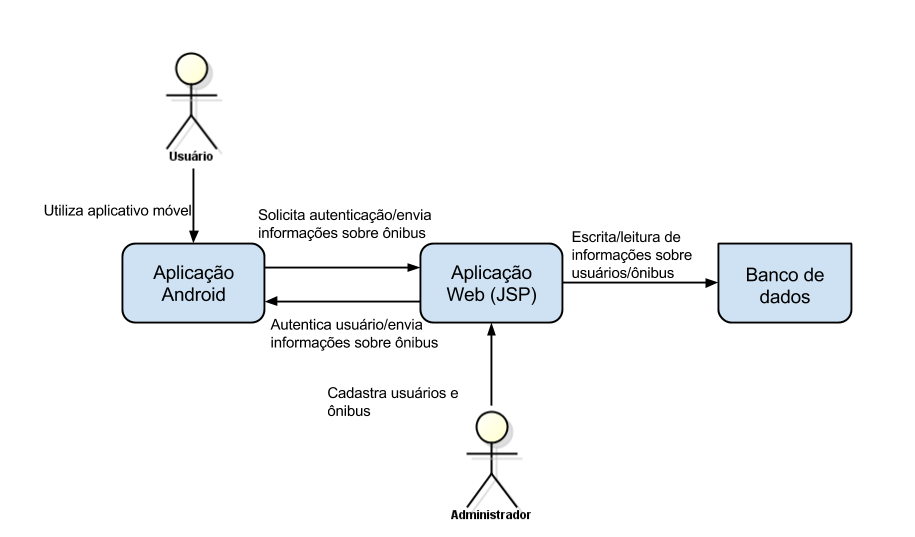
\includegraphics[width=1\columnwidth]{../figs/arquitetura_mbts.png}
    \caption{Arquitetura do MBTS.}Fonte: Adaptado de \citeonline{sujatha}.
    \label{fig:archMBTS}
\end{center}
\end{figure}

Uma limitação do sistema baseado em RF, e percebida pelos próprios autores, diz respeito à distância entre o ônibus e os nós da rede (neste caso os pontos de ônibus). Uma vez que sensores baseados em radio frequência possuem limitações de distância e na transmissão dos dados, acabam limitando a velocidade desenvolvida pelo veículo, o que torna o projeto inviável. 

Ainda, as informações só podem ser coletadas por usuários que já estão próximos ao veículo (ou em pontos de ônibus próximos ao veículo). Isso acaba tirando o propósito de acompanhamento ou rastreio de ônibus, pois o mesmo já está próximo do ponto, e pode ser visualizado por um usuário sem o auxílio de um sistema específico para tal.

\citeonline{alves} apresentaram um sistema -- chamado de \emph{Trip-planner} -- para planejar rotas em tempo real, para pessoas que utilizam transporte público em Lisboa. O sistema consegue informar quais são as melhores rotas e o tempo estimado de viagem para um determinado destino, baseados na estimativa de quantos veículos estão trafegando e quais são suas velocidades.

Informações de tempo-real são coletadas através do GPS equipado nos ônibus. Essas informações são utilizadas em um servidor (o que os autores chamam de \emph{Data Center}) para atualizar históricos e melhorar as estimativas, uma vez que é utilizado um algoritmo para predição de tempos de viagem. Esses históricos se referem à relatórios de quatro meses, com informações sobre tempos de viagem e velocidades dos veículos. Essas informações são analisadas e passam por um classificador, e uma vez processadas, são repassadas para qualquer dispositivo móvel conectados em uma rede sem fio, através de \emph{broadcast} \cite{alves}.

A Figura \ref{fig:archLisbon} descreve de forma simplificada o sistema proposto por \citeonline{alves}. Nota-se claramente que dados históricos e de tempo-real são coletados com o auxílio do GPS instalado no ônibus. Esses dados passam pelo \emph{Data Center} e são utilizados como entrada para um algoritmo de predição. Uma vez processados, distribuem-se os dados para dispositivos móveis através de \emph{broadcast.}

\begin{figure}[h]
\begin{center}
    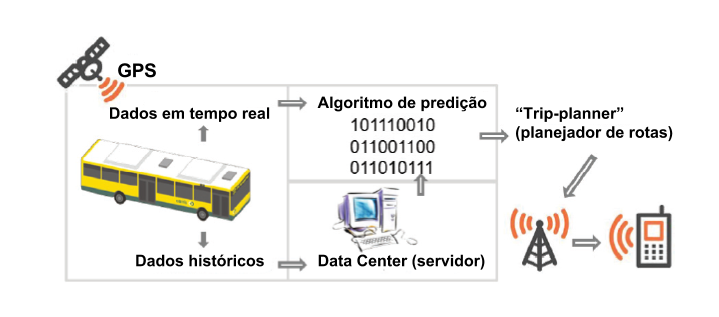
\includegraphics[width=0.85\columnwidth]{../figs/arquitetura_tripplanner.png}
    \caption{Arquitetura do \emph{Trip-planner}.}Fonte: Adaptado de \citeonline{alves}.
    \label{fig:archLisbon}
\end{center}
\end{figure}

\section{Discussões}
% inserir motivação
Conforme já discutido na Introdução, a principal motivação para o desenvolvimento deste projeto é implementar um aplicativo de acompanhamento de ônibus para dispositivos móveis - \textit{smartphones} - que utilize uma rede descentralizada. 

Espera-se que o aplicativo a ser desenvolvido seja de grande ajuda ao dia a dia dos passageiros do transporte coletivo e que, de alguma, forma traga informações de qualidade aos usuários, bem como lhes ofereça uma maior economia de tempo e torne o processo de decisão, sob qual ônibus tomar ou qual rota seguir, descomplicado.

Em termos de arquiteturas de rede, decidiu-se por utilizar neste projeto uma arquitetura que utilize conceitos tanto de DTN quanto de P2P. Acredita-se que os dois mecanismos em conjunto oferecerão uma arquitetura de rede que resultará em alta disponibilidade e boa conectividade a todos os supostos usuários do aplicativo a ser desenvolvido. A união dessas arquiteturas resulta numa arquitetura de rede descentralizada, que não necessita de infra-estrutura de rede e com capacidade de auto-organização, constituindo um modelo muito interessante para ser utilizada por dispositivos que suportam redes móveis e sem fio, como \textit{smartphones} e \textit{tablets}.


%\chapter{Metodologia}\label{cap:metodologia}

Neste capítulo apresenta-se a metodologia a ser empregada a fim de alcançar os desígnios do projeto. Para tanto, apresenta-se de que forma o desenvolvimento será abordado pela equipe e, na sequência, as tecnologias a serem utilizadas, tais como o ambiente de programação, a linguagem de programação, mecanismos para controle de versão e, por fim, a plataforma de software. 

\section{Abordagem da equipe}\label{s:fundamentos}

Partindo de ideias de aplicativos já existentes para acompanhamento de tráfego (Waze) e acompanhamento de ônibus na cidade de Curitiba (Busão Curitibano), a equipe decidiu reuni-las e aperfeiçoá-las em um aplicativo único. O aperfeiçoamento será resultado do uso de arquiteturas de rede que dispensam centralização, como as Redes Tolerantes a Atrasos, (DTN) se contrapondo à arquitetura cliente-servidor, na qual operam softwares (aplicativos) móveis existentes já citados no início desta seção. 

Sendo assim, o uso de uma arquitetura DTN dispensa a necessidade de conectividade contínua para transmissão de informações, uma vez que essa transmissão ocorrerá assim que um usuário, que necessita de informações, esteja próximo de um usuário que porte essas informações. 

Tendo em vista a grande quantidade de usuários que estarão utilizando o aplicativo, e o emprego de uma arquitetura descentralizada como as DTNs, nota-se também a importância da arquitetura Ponto-a-ponto (P2P), que permite que um usuário (que pode ser representado aqui por um nó da rede) adquira um papel simultâneo de "cliente" e "servidor". Em outras palavras, um usuário receberá/enviará informações de/para outros usuários, partindo do princípio que todos estejam utilizando o mesmo aplicativo móvel, a ser desenvolvido neste projeto. A descoberta de outros nós nas proximidades, bem como a propagação de informações por esses nós, dar-se-á de forma transparente ao usuário.

%\subsection{Arquitetura DTN e arquitetura P2P}

%Sistemas \sigla{P2P}{\emph{Peer-to-Peer}} (\emph{Peer-to-Peer}) são capazes de fornecer recursos de rede com sobreposição e auto-organização distribuída, com o intuito de prover uma distribuição eficiente dos dados. O mecanismo básico de funcionamento consiste em pares, nos quais uma entidade presta e ao mesmo tempo consume os recursos oferecidos por outras entidades que compõe o sistema. Outras características que estes sistemas apresentam, normalmente, são auto-organização, tolerância a falhas e escalabilidade \cite{italianos}.

%Em contrapartida, sistemas baseados em \sigla{DTN}{\emph{Delay Tolerant Networks}} (\emph{Delay Tolerant Networks}) são construídos para operar sobre redes sem fio, com múltiplos saltos. A arquitetura visa oferecer conectividade mesmo se uma comunicação fim a fim não exista por um (in)determinado período de tempo e, assim sendo, os nós intermediários da rede devem armazenar os dados até uma nova oportunidade de comunicação seja possível \cite{italianos}.

%Um paradigma típico para as DTNs é o chamado \emph{store-carry-forward} (armazenar, transportar e encaminhar) que consiste na armazenagem de uma mensagem em um nó, o transporte da mesma por este nó e a sua posterior distribuição para outros nós da rede, tão logo surja uma oportunidade para tal \cite{italianos}. Um exemplo simples é exposto na sequência. Supondo que um nó \textbf{S} tenha que se comunicar com um nó \textbf{D}, mas não existe um caminho direto entre os dois; por consequência disso, o nó \textbf{S} terá que armazenar a mensagem. No entanto, \textbf{S} consegue se comunicar com um terceiro nó \textbf{R}, que por sua vez se comunica com o nó \textbf{D}. O nó \textbf{S} pode então encaminhar a mensagem para o nó \textbf{R}, que irá repassá-la para o nó \textbf{D} \cite{italianos}.

%Como consequência dos dois mecanismos apresentados, no escopo deste exposto decidiu-se pelo uso de uma arquitetura de rede que combina os dois modelos apresentados anteriormente. Apesar de algumas disparidades entre os dois paradigmas (a mais notável: operarem em camadas distintas de rede) \cite{italianos}, usar-se-á os dois mecanismos em conjunto a fim de oferecer uma arquitetura de rede decentralizada e com boa conectividade a todos os supostos usuários do aplicativo. Ademais, o fato de ambos trabalharem em ambientes decentralizados, auto-organizados e distribuídos \cite{italianos} tornam-se bastantes interessantes para o escopo do trabalho, já que se encaixa perfeitamente no ambiente em que o aplicativo desenvolvido funcionará. 

%Outra característica interessante, consiste na possibilidade de operação em mecanismos de rede que não são baseados em meios físicos para propagar informações, como Wi-Fi e Bluetooth, por exemplo. Essa possibilidade é ideal para smartphones, dado que uma gama abundante desses aparelhos possui no mínimo um desses recursos disponíveis. 

\section{Tecnologias}\label{s:tecnologias}

A presente seção refere-se às principais tecnologias a serem empregadas no desenvolvimento do projeto, tais como ambientes de desenvolvimento, linguagens de programação, plataforma de software e plataforma de hardware.

\subsection{Ambiente de desenvolvimento}

Pelo fato de o projeto envolver um aplicativo para o sistema operacional Android, é necessário utilizar um ambiente de desenvolvimento específico para essa plataforma.

O \emph{site} oficial para desenvolvimento de aplicativos Android, Android Developers\footnote{O site pode ser acessado em http://developer.android.com/}, disponibiliza algumas ferramentas para a concepção e teste de aplicativos para a plataforma.

É possível utilizar um \emph{plug-in}, juntamente com o Android SDK, e integrá-los em uma instalação existente da conhecida IDE chamada Eclipse, realizando as devidas configurações manualmente. Uma segunda opção, e que torna a preparação do ambiente de desenvolvimento mais simplificada, é baixar um \emph{bundle} que já inclui o Android SDK, a IDE Eclipse, o \emph{plug-in}, ferramentas de desenvolvimento e uma imagem de sistema para emular um dispositivo Android no Desktop. Dessa forma, é possível depurar aplicações Android diretamente no PC, antes de enviá-lo à um dispositivo real. A terceira opção é utilizar uma IDE alternativa chamada \emph{Android Studio}, que atualmente encontra-se em uma versão Beta.

Por experiências dos integrantes com o referido \emph{bundle}, em projetos anteriores, optou-se por utilizar o mesmo no desenvolvimento deste projeto.

Para testes de software será utilizada a emulação do dispositivo Android provida pelo \emph{bundle}, até onde for possível. É dito isso pois o projeto envolve o uso de GPS, Google Maps e compartilhamento de informações entre usuários (\emph{crowdsourcing}), o que não é possível de ser feito apenas com a utilização de um emulador. Dessa forma, será necessário testar a aplicação em um dispositivo real, como um \emph{smartphone} ou um \emph{tablet}, com sistema operacional Android.

\subsection{Linguagem de programação}

Em relação à linguagem de programação, não há a necessidade de fazer um levantamento dentre as linguagens de programação existentes atualmente e escolher qual será a mais adequada ao projeto. Uma vez que o projeto tem como foco o desenvolvimento de uma aplicação Android, é mandatório que a mesma seja desenvolvida utilizando a linguagem de programação Java juntamente com a API (que contém bibliotecas e ferramentas) incluída no Android SDK. A princípio, não será utilizada nenhuma biblioteca de terceiros (\emph{third-party}).

\subsection{Controle de Versão}

Será utilizado um sistema de controle de versão (\sigla{CVS}{\emph{Control Version System}}, \emph{Control Version System}) para o versionamento do código-fonte do aplicativo Android. Vários são os sistemas de versionamento de arquivos, dentre os quais os mais comuns são o SVN e Git. Para este último, existem repositórios de código-fonte gratuitos, como o GitHub (https://github.com) e o BitBucket (https://bitbucket.org).

O ideal seria manter um servidor próprio com o SVN ou o Git instalados. No entanto, isso poderia envolver custos adicionais, pois seria necessário deixar uma máquina dedicada para o controle de versão e acessível para todos os integrantes do projeto, além de realizar \emph{backups} periódicos.

O GitHub permite que qualquer pessoa crie uma quantidade ilimitada de repositórios gratuitamente e compartilhe-o com quantos colaboradores for necessário. No entanto, o código-fonte fica disponível publicamente, para qualquer um acessar. Para projetos acadêmicos (como TCCs, teses de mestrado e doutorado), isso pode não ser indicado. O GitHub também oferece repositórios privados, com acesso restrito, mas apenas a partir da assinatura de um plano.

Em contrapartida, o BitBucket oferece uma quantidade ilimitada de repositórios privados gratuitamente, permitindo até cinco colaboradores em um projeto. Como o projeto é constituído de dois integrantes e levantou-se a necessidade de versionar o código-fonte sem disponibilizá-lo publicamente, optou-se por utilizar o BitBucket como repositório de código-fonte e o Git como como sistema de controle de versão.

\subsection{Plataforma de software}

Em relação ao sistema operacional Android, levanta-se outra questão. O Android, como sistema operacional, possui diversas versões desde o seu lançamento. Cada uma dessas versões acaba por incluir novas funcionalidades não apenas para o usuário final, mas também, para os desenvolvedores. É certo que existe a chamada retrocompatibilidade, que permite que a grande maioria das aplicações desenvolvidas para uma versão mais recente do S.O., execute sem maiores problemas em uma versão mais antiga. No entanto, para que isso ocorra, muitas vezes a aplicação fica limitada, pois o desenvolvedor é forçado à desabilitar certos recursos que não são compatíveis, de forma alguma, com versões mais antigas da plataforma.

No momento da escrita desta proposta, a versão mais recente do Android é a versão 4.4 (KitKat). A maioria dos dispositivos disponíveis no mercado -- \emph{smartphones} e \emph{tablets} -- possuem uma versão do Android 4.0+ instalada. A mais recente versão do S.O., a versão 5.0 (Lollipop), está prestes a ser lançada, e apenas alguns poucos dispositivos já existentes no mercado receberão a atualização para o novo sistema.

A Tabela \ref{tab:marketShare} fornece informações referentes ao \emph{market share} das versões do Android, desde a 2.2 (Froyo) até a 4.4 (KitKat). Os dados foram coletados através da aplicação Google Play Store em um período de sete dias, finalizando no dia 03 de novembro de 2014. É possível verificar o percentual de quantos dispositivos executam uma determinada versão do sistema operacional. Essas informações são úteis para que o desenvolvedor determine qual versão da plataforma terá como ``alvo''.

\begin{table}[h!]
%Se o nome da tabela for muito grande, é possível colocar entre colchetes o título reduzido que será mostrado na lista de tabelas e entre aspas o título completo que será mostrado acima da tabela. O mesmo é válido para figuras.

\caption[Market Share das versões do Android]{Market Share das versões do Android. Fonte: \cite{androidDevDashboards}}
\begin{center}
%\scalebox{0.75}{
\begin{tabular}{|c|c|c|c|}
\hline
\textbf{Versão}     &\textbf{Codinome}      & \textbf{API}      &\textbf{Distribuição} \\ \hline \hline
2.2                 & Froyo                 & 8                 & 0,6$\%$	\\
2.3.3 - 2.3.7       & Gingerbread           & 10                & 9,7$\%$	\\
4.0.3 - 4.0.4       & Ice Cream Sandwich    & 15                & 8,5$\%$	\\
4.1.x               & Jelly Bean            & 16                & 22,8$\%$	\\
4.2.x               & Jelly Bean            & 17                & 20,8$\%$	\\
4.3                 & Jelly Bean            & 18                & 7,3$\%$	\\
4.4                 & KitKat                & 19                & 30,2$\%$	\\ \hline
\end{tabular}%}
\end{center}
\label{tab:marketShare}
\end{table}

Observa-se na tabela que cerca de 10,4$\%$ usuários usa um dispositivo com uma versão antiga da plataforma, de codinome Froyo (2.2) ou Gingerbread (2.3.3 - 2.3.7). Uma parcela ainda menor utiliza as versões Ice Cream Sandwich (4.0.3 - 4.0.4), 8,5$\%$. Grande parte dos usuários -- cerca de 50$\%$ -- utiliza o Android Jelly Bean (4.1.x - 4.3) e 30,2$\%$ utiliza a última versão lançada, KitKat (4.4).

Portanto, devido à popularidade da versão Jelly Bean (4.1.x - 4.3) do sistema operacional Android, o desenvolvimento do projeto terá como foco dispositivos que executam, no mínimo, esta versão da plataforma.

\subsection{Plataforma de hardware}

Para o projeto em questão não será necessária a utilização de uma plataforma de hardware, pois a aplicação executará diretamente sobre um dispositivo móvel, tal como um \textit{smartphone} ou um \textit{tablet}.

\section{Etapas de desenvolvimento}

Inicialmente será feito um estudo das APIs disponíveis no Android SDK, e um levantamento para detectar se há a necessidade de utilizar APIs de terceiros (\textit{third-party}). 

Com os diagramas UML já projetados, será preparado o ambiente de desenvolvimento, realizando-se o \textit{download} do \textit{bundle}, instalação de \textit{drivers} para depuração em um dispositivo móvel real via cabo USB e configurações necessárias. Na sequência, dar-se-á início à implementação da aplicação.

Inicialmente, os testes serão realizados no emulador Android, disponibilizado pelo \textit{bundle}, conforme citado na seção anterior. Testes mais complexos serão feitos em um dispositivo real (\textit{smartphone} e/ou \textit{tablet}) que execute o sistema operacional Android com versão 4.1.x, pelo menos. Ressalta-se que não será necessária aquisição deste(s) dispositivo(s), uma vez que os próprios integrantes do projeto os possuem.
%\chapter{Recursos de Hardware e Software}\label{cap:recursos}

O presente capítulo menciona os recursos de \textit{hardware} e \textit{software} necessários para o desenvolvimento do projeto.

\section{Recursos de Hardware}\label{s:hardware}

Uma vez que o projeto diz respeito à uma aplicação Android que executará sobre um dispositivo móvel (\textit{smartphones} e \textit{tablets}), não é necessário a compra e/ou o uso de componentes de hardware (microcontroladores, circuitos integrados, fontes de alimentação, bateria, entre outros) para o desenvolvimento do projeto.

%Indique aqui os recursos de hardware como componentes digitais, analógicos, fontes de alimentação, baterias, sensores, atuadores, entre outros. Especifique a origem dos recursos de hardware.

\section{Recursos de Software}\label{s:software}

%Devem ser apresentados aqui os recursos de software, incluindo os principais fundamentos (teorias, algoritmos, paradigmas) e tecnologias (ambientes de desenvolvimento, linguagens de programação) a serem empregados. Especifique a origem dos recursos de software.

Os recursos de software englobam ambientes de desenvolvimento, linguagem de programação e plataformas de software.

Conforme citado no capítulo anterior, para a programação e teste da aplicação Android será utilizado o ambiente de desenvolvimento \textbf{Eclipse ADT}, que nada mais é que um \textit{bundle} (pacote) que inclui diversos componentes necessários para a concepção do aplicação. Segundo o site oficial para desenvolvimento de aplicações Android, \citeonline{androidDevSDK}, os componentes inclusos são os seguintes:

\begin{itemize}
\item Ambiente de desenvolvimento Eclipse + \textit{plugin} \sigla{ADT}{\textit{Android Developer Tools}} (\textit{Android Developer Tools});
\item Android \sigla{SDK}{\textit{Software Development Kit}} (\textit{Software Development Kit});
\item Ferramentas adicionais para a plataforma Android;
\item Uma versão da plataforma Android (geralmente a mais recente);
\item Uma versão da imagem do sistema Android para o emulador.
\end{itemize}

É possível realizar o \textit{download} do \textit{bundle} gratuitamente no Android Developers, no seguinte link: \url{http://developer.android.com/sdk/index.html}. Há versões disponíveis para Windows e Linux, tanto 32-bit quanto 64-bit. Para Mac OS X, apenas a versão 64-bit encontra-se disponível.

% Verificar
%O \textit{bundle} também inclui a versão mais recente do JDK, necessário para a compilação de aplicativos na linguagem Java. 

Segundo \citeonline{garySims}, a linguagem de programação ``oficial'' para o desenvolvimento de aplicações Android é Java. Grande parte das aplicações são escritas em Java e suas \sigla{API}{\textit{Application Programming Interface}} (\textit{Application Programming Interface}) são projetadas para serem chamadas primeiramente por Java. É possível desenvolver utilizando linguagens como C e C++, mas isso é algo que a própria Google, desenvolvedora do Android, não incentiva \cite{garySims}.

Pode-se fazer o \textit{download} de várias versões do \sigla{JDK}{\textit{Java Development Kit}} (\textit{Java Development Kit}) gratuitamente a partir do site oficial da Oracle: \url{http://oracle.com}. O JDK é necessário para a compilação de aplicativos na linguagem Java e por consequência, o Eclipse ADT irá utilizá-lo juntamente com o Android SDK para compilação da aplicação Android.

Durante todo o desenvolvimento do projeto, será utilizado o Git como sistema de controle de versão, conforme citado no capítulo anterior. Será criado um repositório privado no BitBucket (\url{https://bitbucket.org}) para código-fonte da aplicação Android. Outro repositório foi criado no GitHub (\url{https://github.com}) para o ``versionamento'' desta proposta, que está sendo escrita em LaTeX. A criação dos repositórios, tanto no BitBucket quanto no GitHub, é gratuita.

Por fim, a plataforma de \textit{software} sobre a qual executará a aplicação Android, é o próprio sistema operacional Android, disponível em diversos \textit{smartphones} e \textit{tablets} existentes no mercado. Conforme estudo apresentado no capítulo anterior, o desenvolvimento da aplicação Android terá como foco sistemas operacionais que executam, no mínimo, a versão 4.1.x (Jelly Bean).
%\chapter{Viabilidade e Cronograma Preliminar}\label{cap:viabilidade}

Apresente aqui a viabilidade e o cronograma preliminar do projeto.

\section{Viabilidade}\label{s:viabilidade}

Relate a viabilidade técnica e financeira do projeto.

\section{Cronograma Preliminar}\label{s:cronograma}

Identifique e liste as etapas necessárias para o seu projeto.
Ordene as etapas em ordem cronológica, indicando o tempo de duração suposto para cada etapa.
%\chapter{Contexto}\label{cap:contexto}

O Contexto do projeto se aplica à cidade de Curitiba, em especial aos usuários de transporte público da cidade, haja vista que o aplicativo visa informar, com a maior precisão possível, a localização dos automóveis que operam em uma determinada linha de ônibus. 

Apesar do caráter altruísta do projeto, o mesmo desenvolver-se-á sem qualquer ligação externa aos elementos do grupo ou fora do ambiente da UTFPR. Logo, é um aplicativo de propósito independente, mas com foco voltado à população em geral. 

Como consequência, a alocação de recurso destinados ao progresso do  projeto será de responsabilidade de seus desenvolvedores, exclusivamente, assim como a responsabilidade por sua construção.


%\chapter{Conclusão}\label{cap:conclusao}

Sabe-se que transporte coletivo é um tema em voga na maioria das cidades brasileiras, e também é uma área na qual aloca-se grande quantidade de recursos. Em especial, na cidade de Curitiba, tida por muitos anos como possuidora do melhor transporte público do país, há uma preocupação grande nesse aspecto. 

Ao longo do ano é possível visualizar por toda cidade, campanhas publicitárias voltadas para esse propósito, tendo em vista conscientizar o usuário do transporte coletivo acerca de alguns comportamentos, e também, tentando melhorar a qualidade do serviço prestado. Verifica-se também  que as tentativas de melhora do transporte coletivo não partem apenas da prefeitura da cidade, como  documentou-se nesse exposto, um grupo de desenvolvedores buscou materializar um aplicativo que mostrasse, em tempo real, a localização de cada ônibus em uma(s) determinada(s) linha(s) de interesse. No entanto, a aplicação apresentava um funcionamento um tanto instável, já que dependia dos serviços de um servidor da URBS para seu funcionamento correto. 

Numa tratativa que visa resolver esse problema, elaborou-se um projeto com intuito de elaborar um aplicativo que funcione sob uma arquitetura \textit{ad-hoc} e utilize recursos disponíveis em um \textit{smartphone}, e portanto, presente no dia a dia da  maioria dos usuários de ônibus na cidade. Entretanto, na acepção da proposta de projeto, encontrou-se certa dificuldade em definir o que o aplicativo ia fazer, quais seriam os recursos existentes no programa e principalmente, a forma de propagar a informação que faria o sistema, como um todo, funcionar. 

A escolha para a arquitetura de rede foi pensada de modo a aliar conceitos de DTN e P2P. A priori, a ideia apresentou-se confusa, já que as duas abstrações parecem paradoxais, todavia, existem registros na literatura de algoritmos que funcionam com essas características. Passados esses questionamentos iniciais o projeto progrediu de forma tranquila. A equipe trabalhou em conjunto quase na totalidade do tempo, o que facilitou a tomada de decisões e resolução de conflitos. 

No que tange projetos futuros, um enfoque interessante que poderia ser discutido apoia-se num mecanismo que garanta algum tipo de redundância na rede de comunicação. De certa forma, isso suportaria um prisma egrégio do projeto que é a atualização das informações em tempo real, ou seja, se uma abordagem falhar, existiria outra para garantir a propagação dos dados em um tempo exequível. Outra singularidade consiste em tornar acessíveis aos usuários, todas as linhas de ônibus cadastradas na URBS, sejam elas metropolitanas ou urbanas, de forma que haja cobertura total de informações em toda a cidade.

Por fim, busca-se com esse projeto fornecer um mecanismo de fácil manipulação e que traga benefícios à população em geral.
%%---------- Referencias ----------

\chapter{Referências Bibliográficas}

Todas as referências citadas no texto devem estar relacionadas em ordem alfabética. \textbf{Ao utilizar o Latex, as referências são ordenadas automaticamente.}

Referências não citadas no texto do documento, não devem ser apresentadas na lista de Referências Bibliográficas.

As normas da ABNT para referências bibliográficas podem ser consultadas em \cite{NormasUTFPR}.

Para citar referências no texto utilizando o latex, use o comando $citeonline$ ou $cite$, precedido de uma barra invertida.

Com o comando $citeonline\{vendramin2012\}$, a impressão no texto ficará da seguinte forma:

Vendramin (2012).

Ou seja, a citação aparece inserida dentro do texto, como por exemplo:

Conforme a autora Vendramin (2012), a proposta de TCC ...

Ao usar o comando $cite\{vendramin2012\}$, a impressão no texto ficará da seguinte forma:

A proposta de TCC ... (Vendramin, 2012).

A seguir são apresentados exemplos de referências bibliográficas criadas no Latex. As referências são inseridas em um arquivo .bib e o nome desse arquivo (por exemplo, Referencias) deve ser usado ao chamar o comando $bibliography\{Referencias\}$ precedido por uma barra invertida. O comando $bibliography$ é responsável por gerar de forma automática, a partir do arquivo $Referencias.bib$, as referências bibliográficas citadas no documento.

\textbf{Livros}

Para exemplos de como referenciar livros veja as seguintes referências: \cite{castro2006} e \cite{ENGELBRECHT2007}.

\textbf{Artigos de Periódicos}

Para exemplos de como referenciar artigos de periódicos veja as seguintes referências: \cite{vendramin2012a} e \cite{cao2012}.

\textbf{Relatórios Técnicos e Normas Técnicas}

Para exemplos de como referenciar relatórios técnicos ou normas técnicas veja as seguintes referências: \cite{mills2004} e \cite{RFC5050}.

\textbf{Artigos Científicos em Congressos/Conferências/Simpósios}

Para exemplos de como referenciar artigos científicos veja as seguintes referências: \cite{vendramin2012b} e \cite{vendramin2011}.

\textbf{Monografias/Dissertações/Teses}

Para exemplos de como referenciar monografias, dissertações ou teses veja as seguintes referências: \cite{vendramin2012c} e \cite{saleem2001}.

\bibliography{referencias}

%---------- Apêndices e Anexos ----------
% Apêndice
%\appendix
%\chapter{Título do Apêndice}

Elemento opcional, que consiste em texto ou documento \textbf{elaborado pelo autor}, a fim de complementar sua argumentação, sem prejuízo da unidade nuclear do trabalho.

Os apêndices devem ser identificados por letras maiúsculas consecutivas, seguidas de travessão e respectivo título.

% Anexo
%\appendix
%\renewcommand{\appendixname}{Anexo} % Para criar Anexo ao invés de Apêndice
%\chapter{Título do Anexo}

Elemento opcional, que consiste em texto ou documento \textbf{não elaborado pelo autor}, que serve de fundamentação, comprovação e ilustração.

Os anexos devem ser identificados por letras maiúsculas consecutivas, seguidas de travessão e respectivo título.

\end{document}